\subsubsection{Mobile Client}\label{subsec:mobile-client-realisation}

Dieses Kapitel zeigt die umgesetzten Ansichten des Mobile Clients.
Weitere Informationen zur Bedienung des Mobile Clients sind dem Benutzerhandbuch zu entnehmen\footnote{Siehe Anhang C}.

\subsubsection*{Anmeldung und Konfiguration}

Wird die Mobile Client Applikation zu ersten Mal geöffnet, muss die korrekte Konfiguration geladen werden.
So können Buttons für die benötigten Benachrichtigungen angezeigt und relevante Benachrichtigungen empfangen werden.
In einem ersten Schritt wird dem Benutzer deshalb eine einfache Login-Maske angezeigt.
Darin kann sich der Benutzer mit Benutzername und Passwort anmelden.
War die Anmeldung erfolgreich, werden alle Konfigurationen geladen, die dem Benutzer zur Verfügung stehen.
Die verfügbaren Konfigurationen werden dem Benutzer in einer Liste angezeigt und er wird aufgefordert, die gewünschte Konfiguration auszuwählen.
Nachdem die Auswahl erfolgt ist, wird der Benutzer zur Startseite weitergeleitet.

\begin{figure}[h]
    \centering
    \begin{minipage}[b]{0.4\textwidth}
        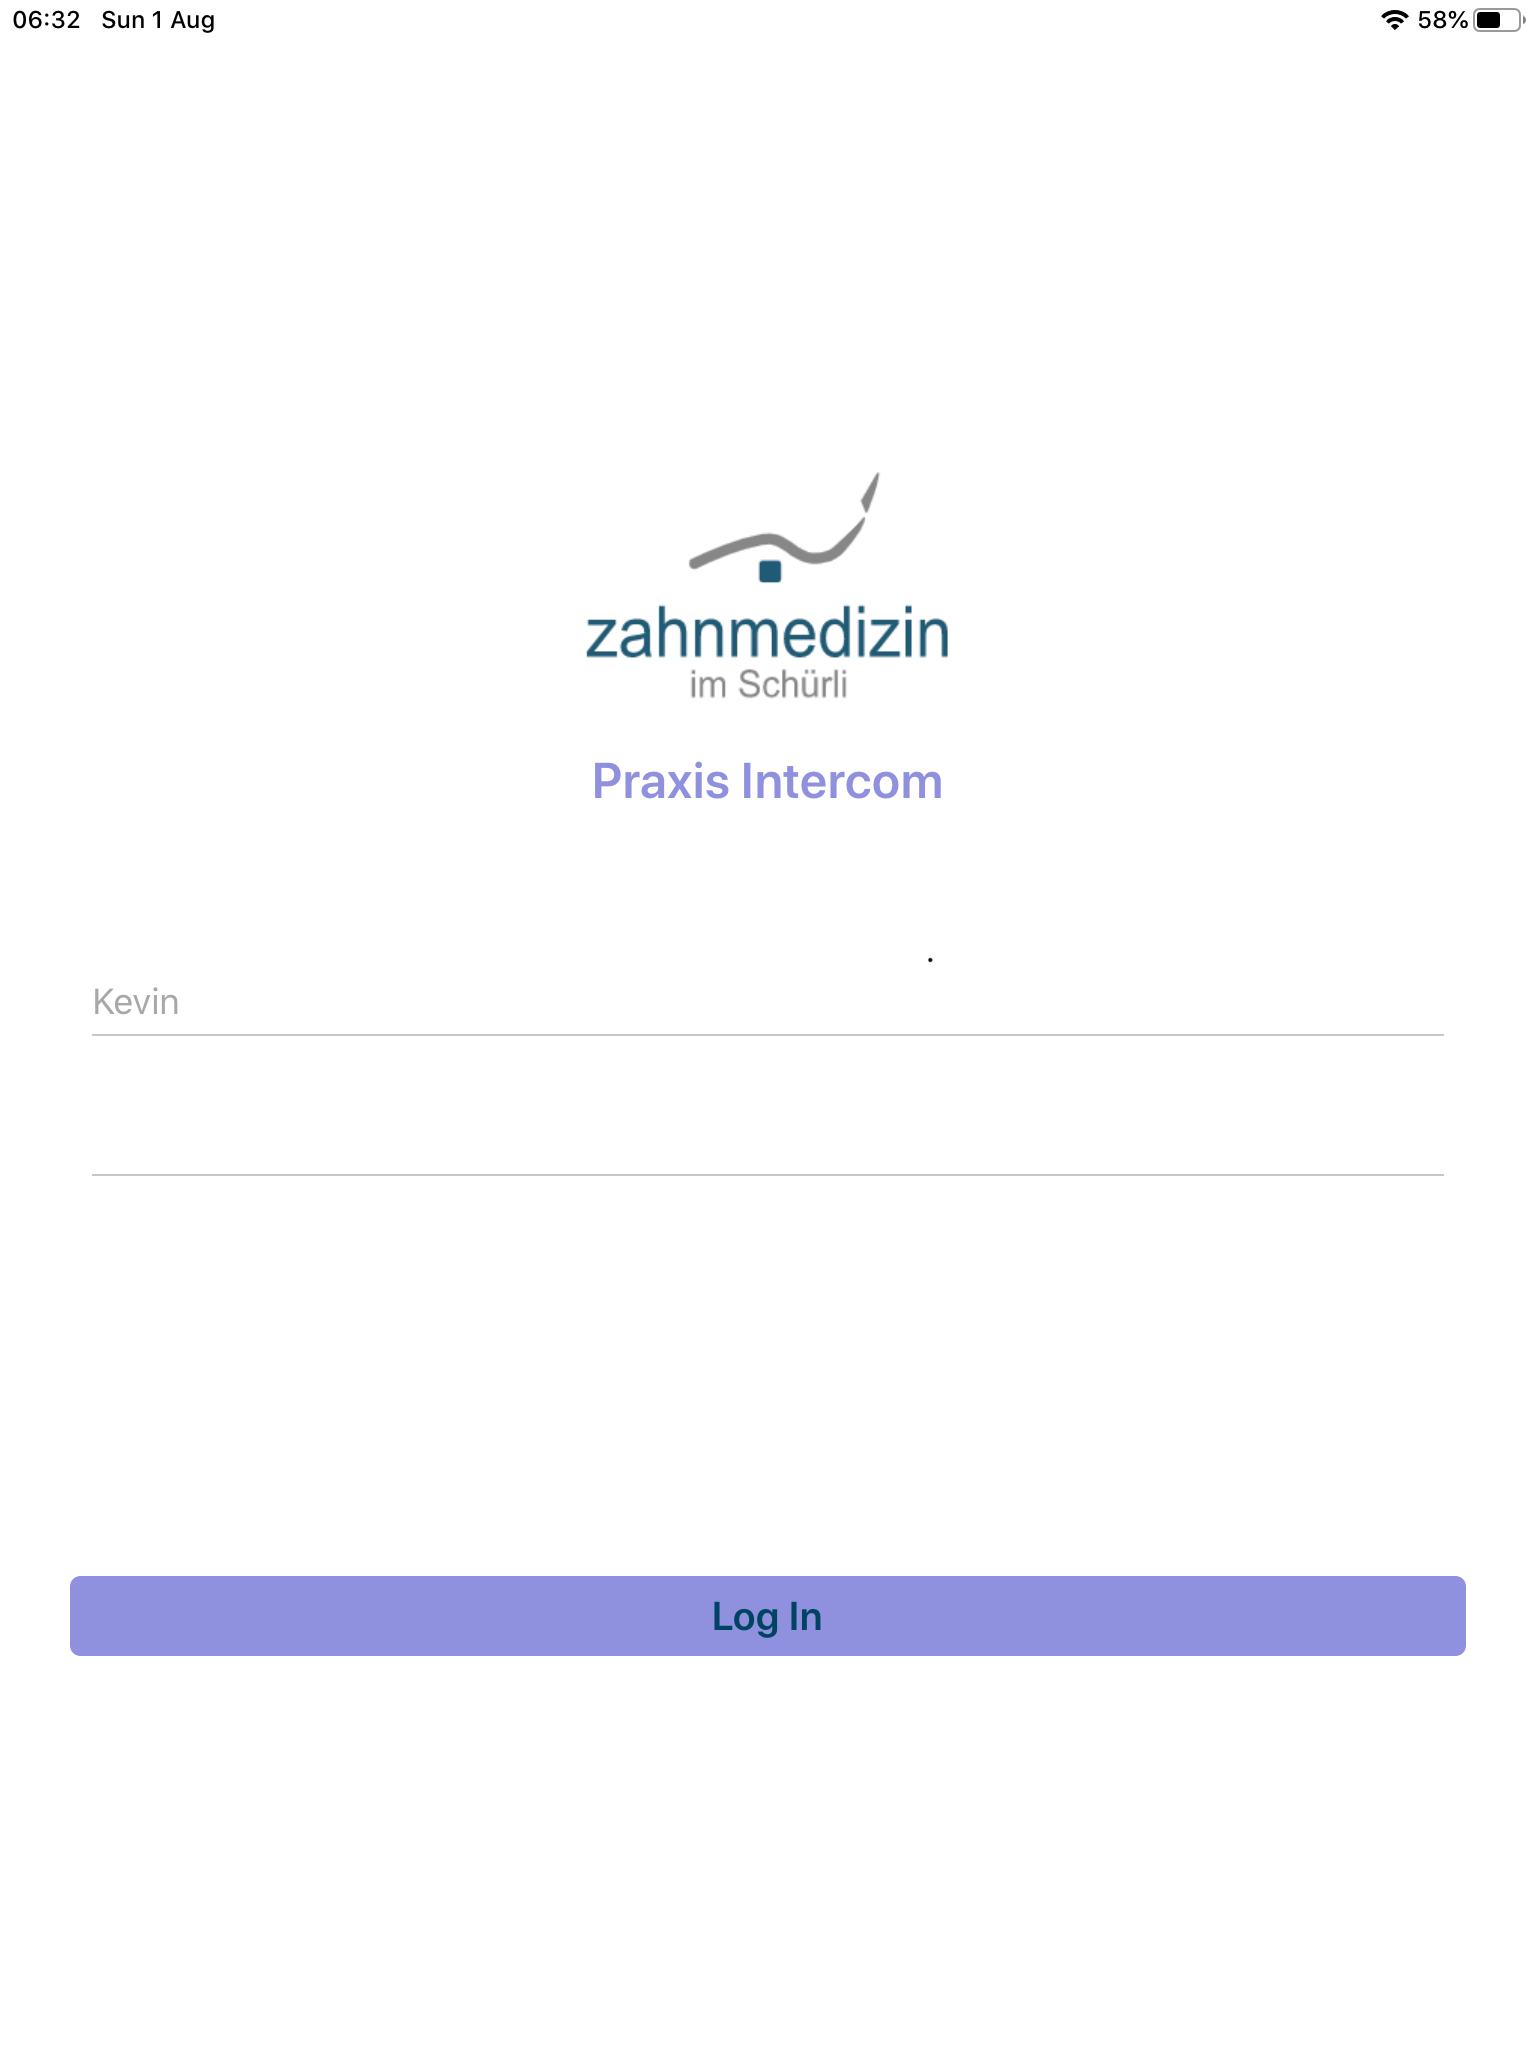
\includegraphics[width=\textwidth]{graphics/screenshots/mobileclient/screenshots-login}
        \caption{Login}
    \end{minipage}
    \hfill
    \begin{minipage}[b]{0.4\textwidth}
        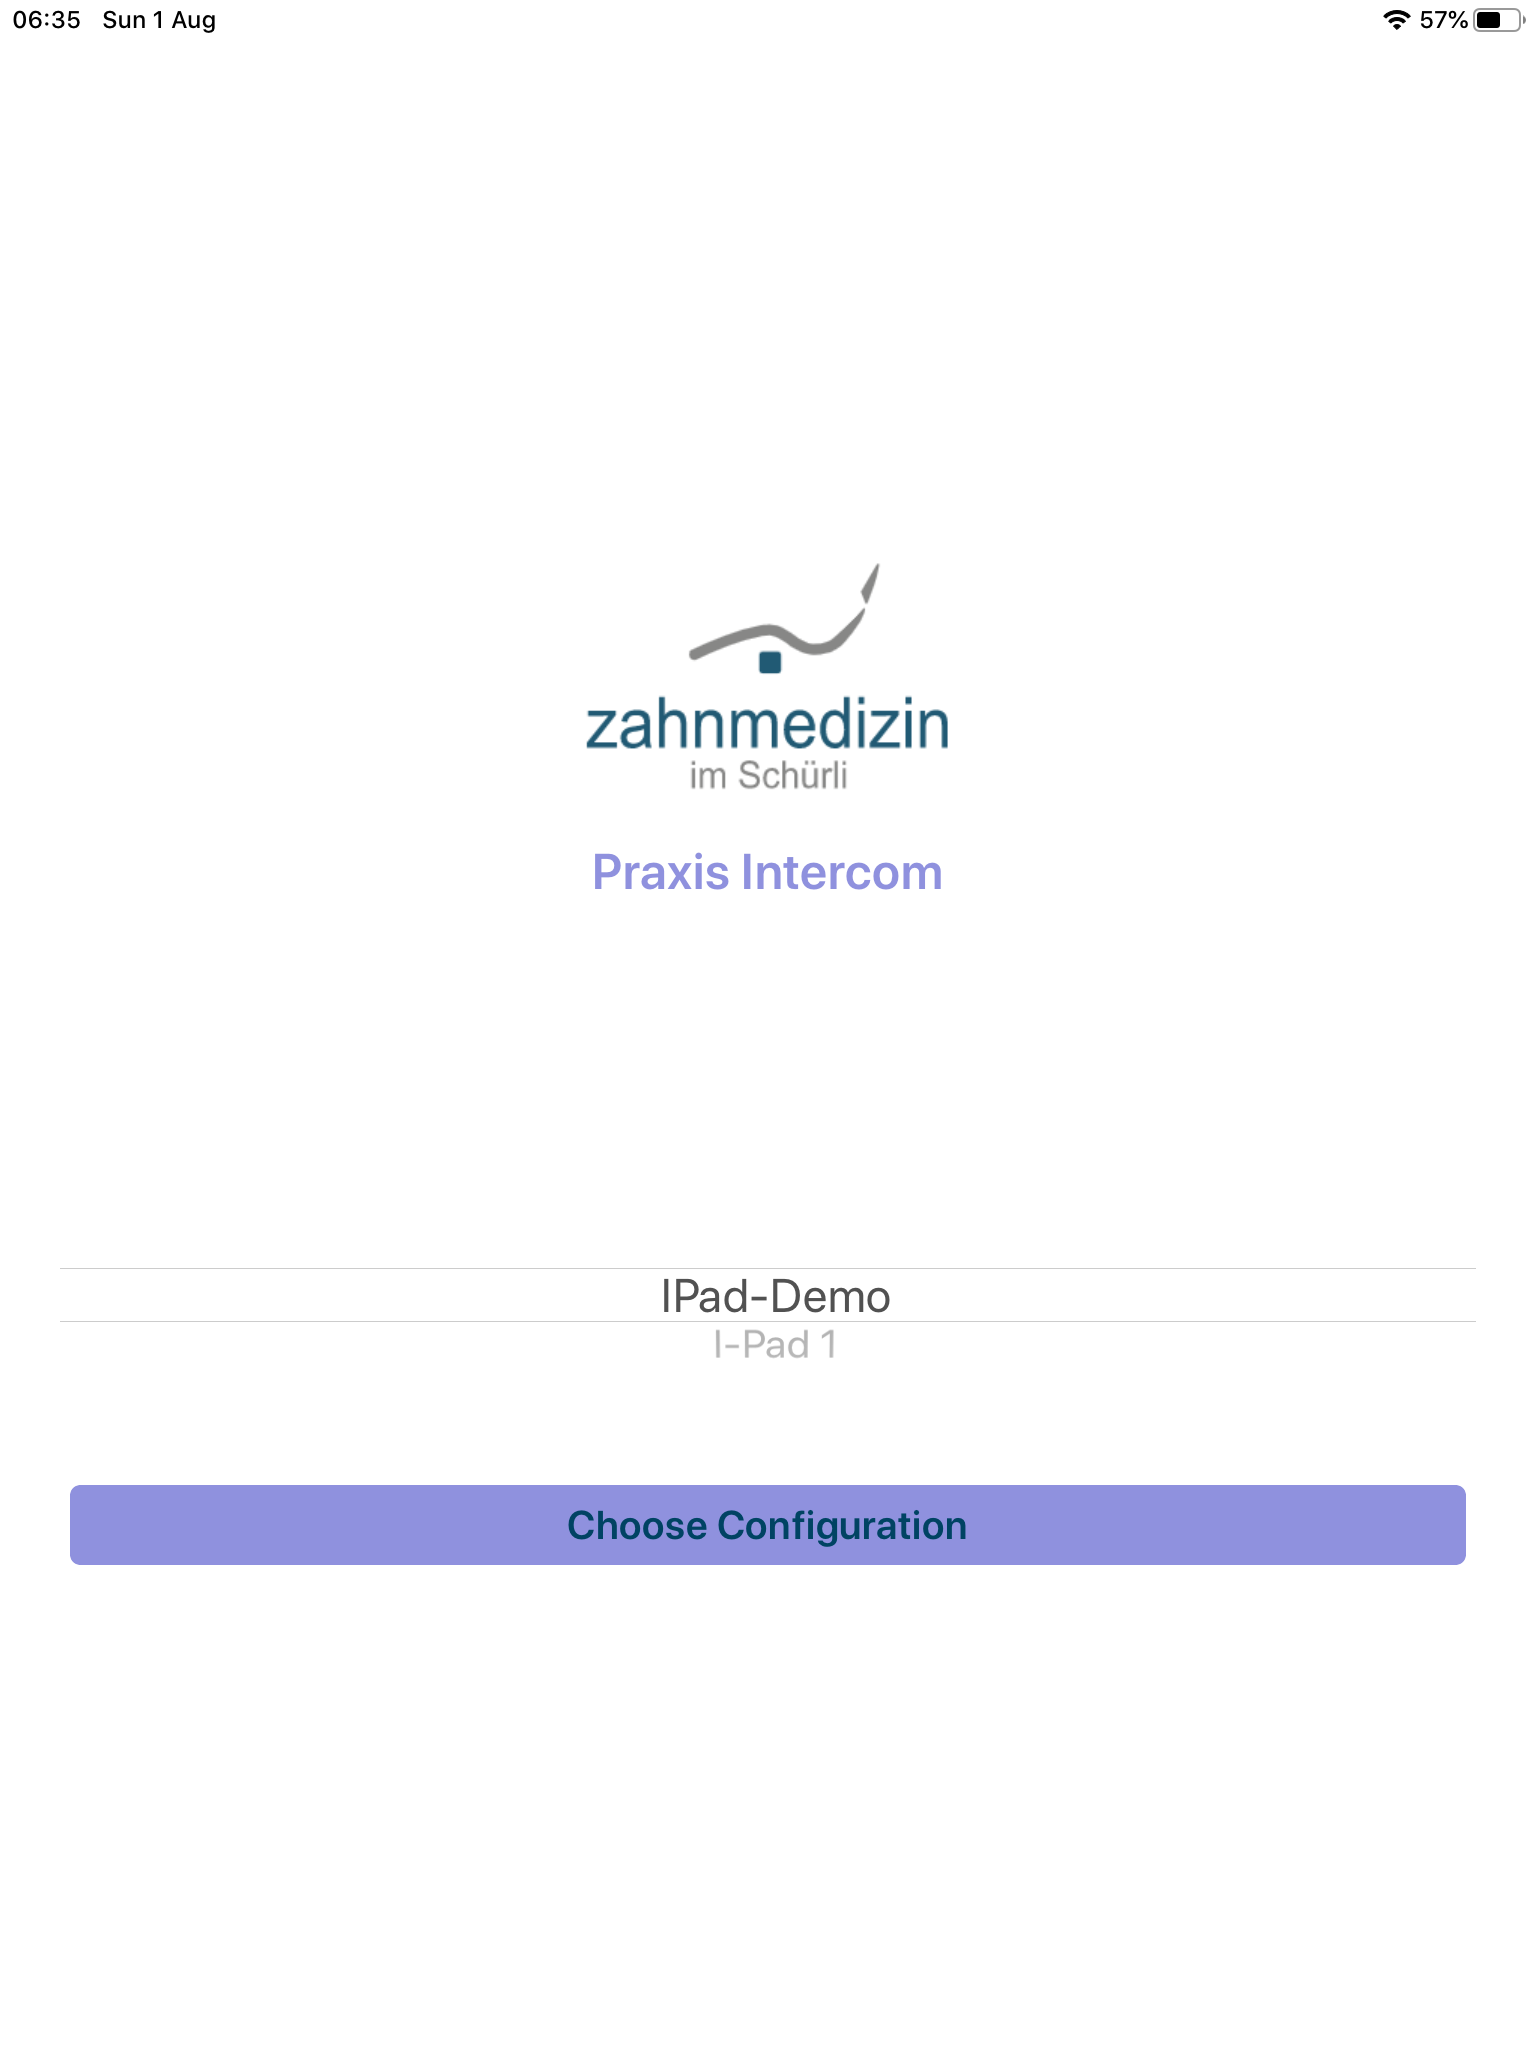
\includegraphics[width=\textwidth]{graphics/screenshots/mobileclient/screenshot-select-config}
        \caption{Konfiguration}
    \end{minipage}
    \label{fig:MobileClient-Screens1}
\end{figure}

\clearpage

\subsubsection*{Benachrichtigungen versenden}

Im Tab Home der Startseite werden Buttons angezeigt, um Benachrichtigungen zu versenden.
Die Buttons werden dynamisch aus der geladenen Konfiguration generiert.
Dabei gibt die Konfiguration den Text vor, der auf dem Button angezeigt wird.
Der Inhalt der Benachrichtigung, die der Button auslöst, ist in der Konfiguration im Cloud Service hinterlegt.

Tippt der Benutzer auf einen der Buttons, wird die entsprechende Benachrichtigung versendet.
Die Vermittlung, an die relevanten Empfänger übernimmt dabei der Cloud Service.
Dieser entscheidet anhand der vorhandenen Konfiguration, welchen Clients die Benachrichtigung zugestellt wird.
Schlägt das Versenden der Benachrichtigung an mindestens einen Empfänger fehl, wird dies dem Benutzer angezeigt.
Der Benutzer hat dann die Möglichkeit, das Versenden an diese Empfänger wiederholen.

\begin{figure}[h]
    \centering
    \begin{minipage}[b]{0.4\textwidth}
        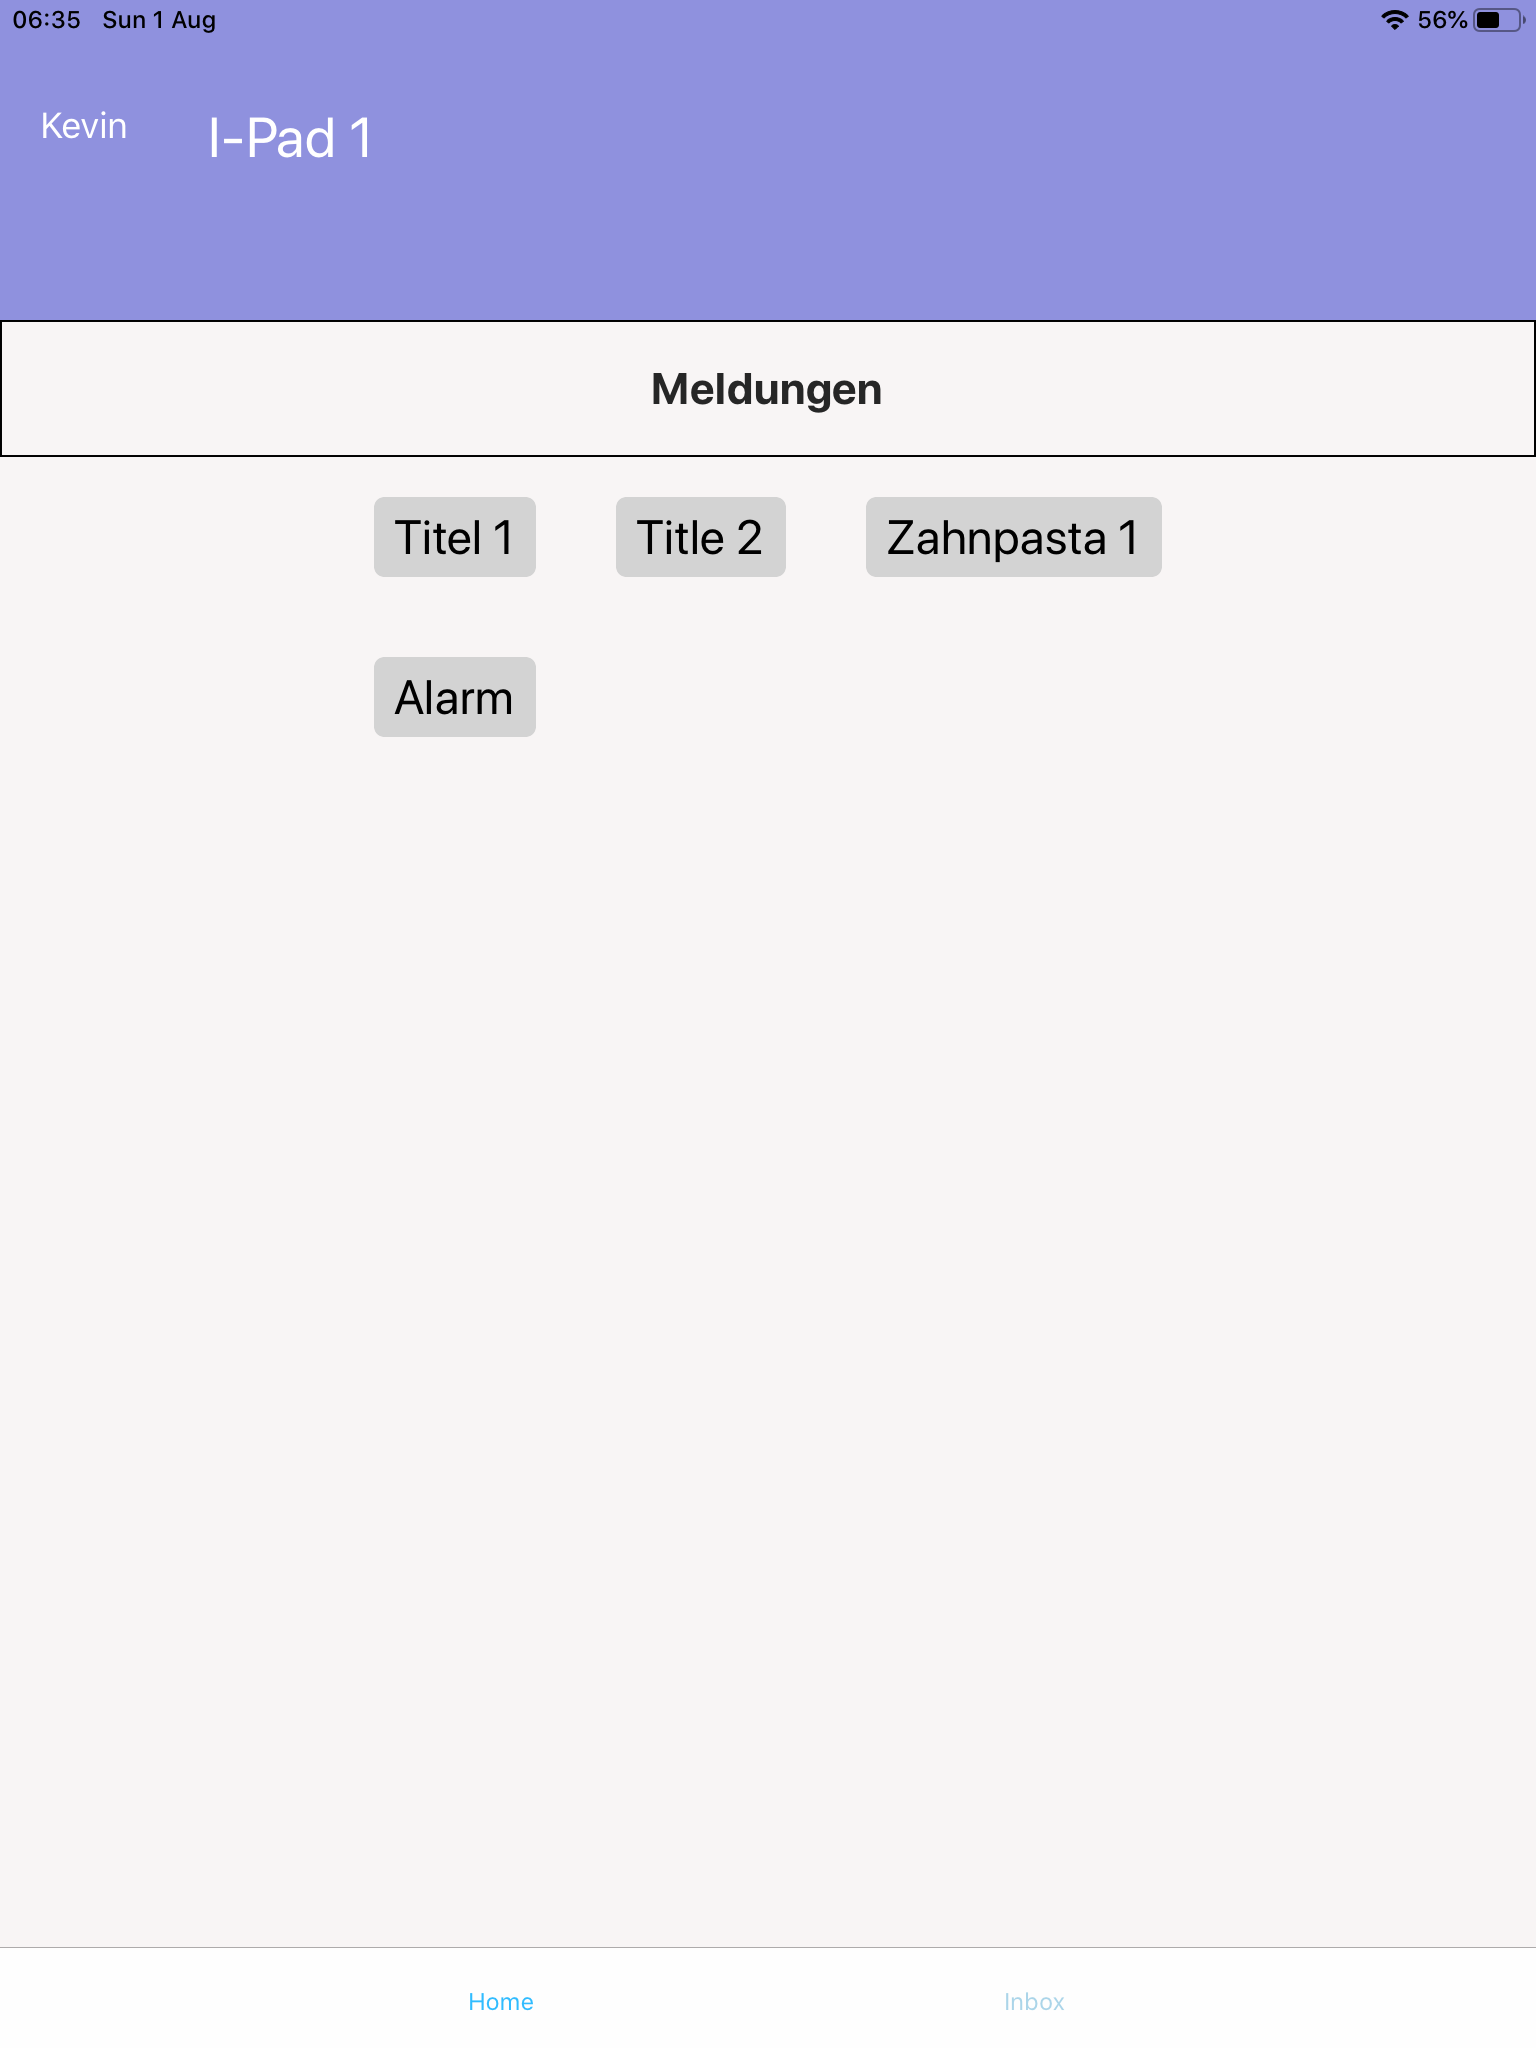
\includegraphics[width=\textwidth]{graphics/screenshots/mobileclient/screenshot-homescreen}
        \caption{Home}
    \end{minipage}
    \hfill
    \begin{minipage}[b]{0.4\textwidth}
        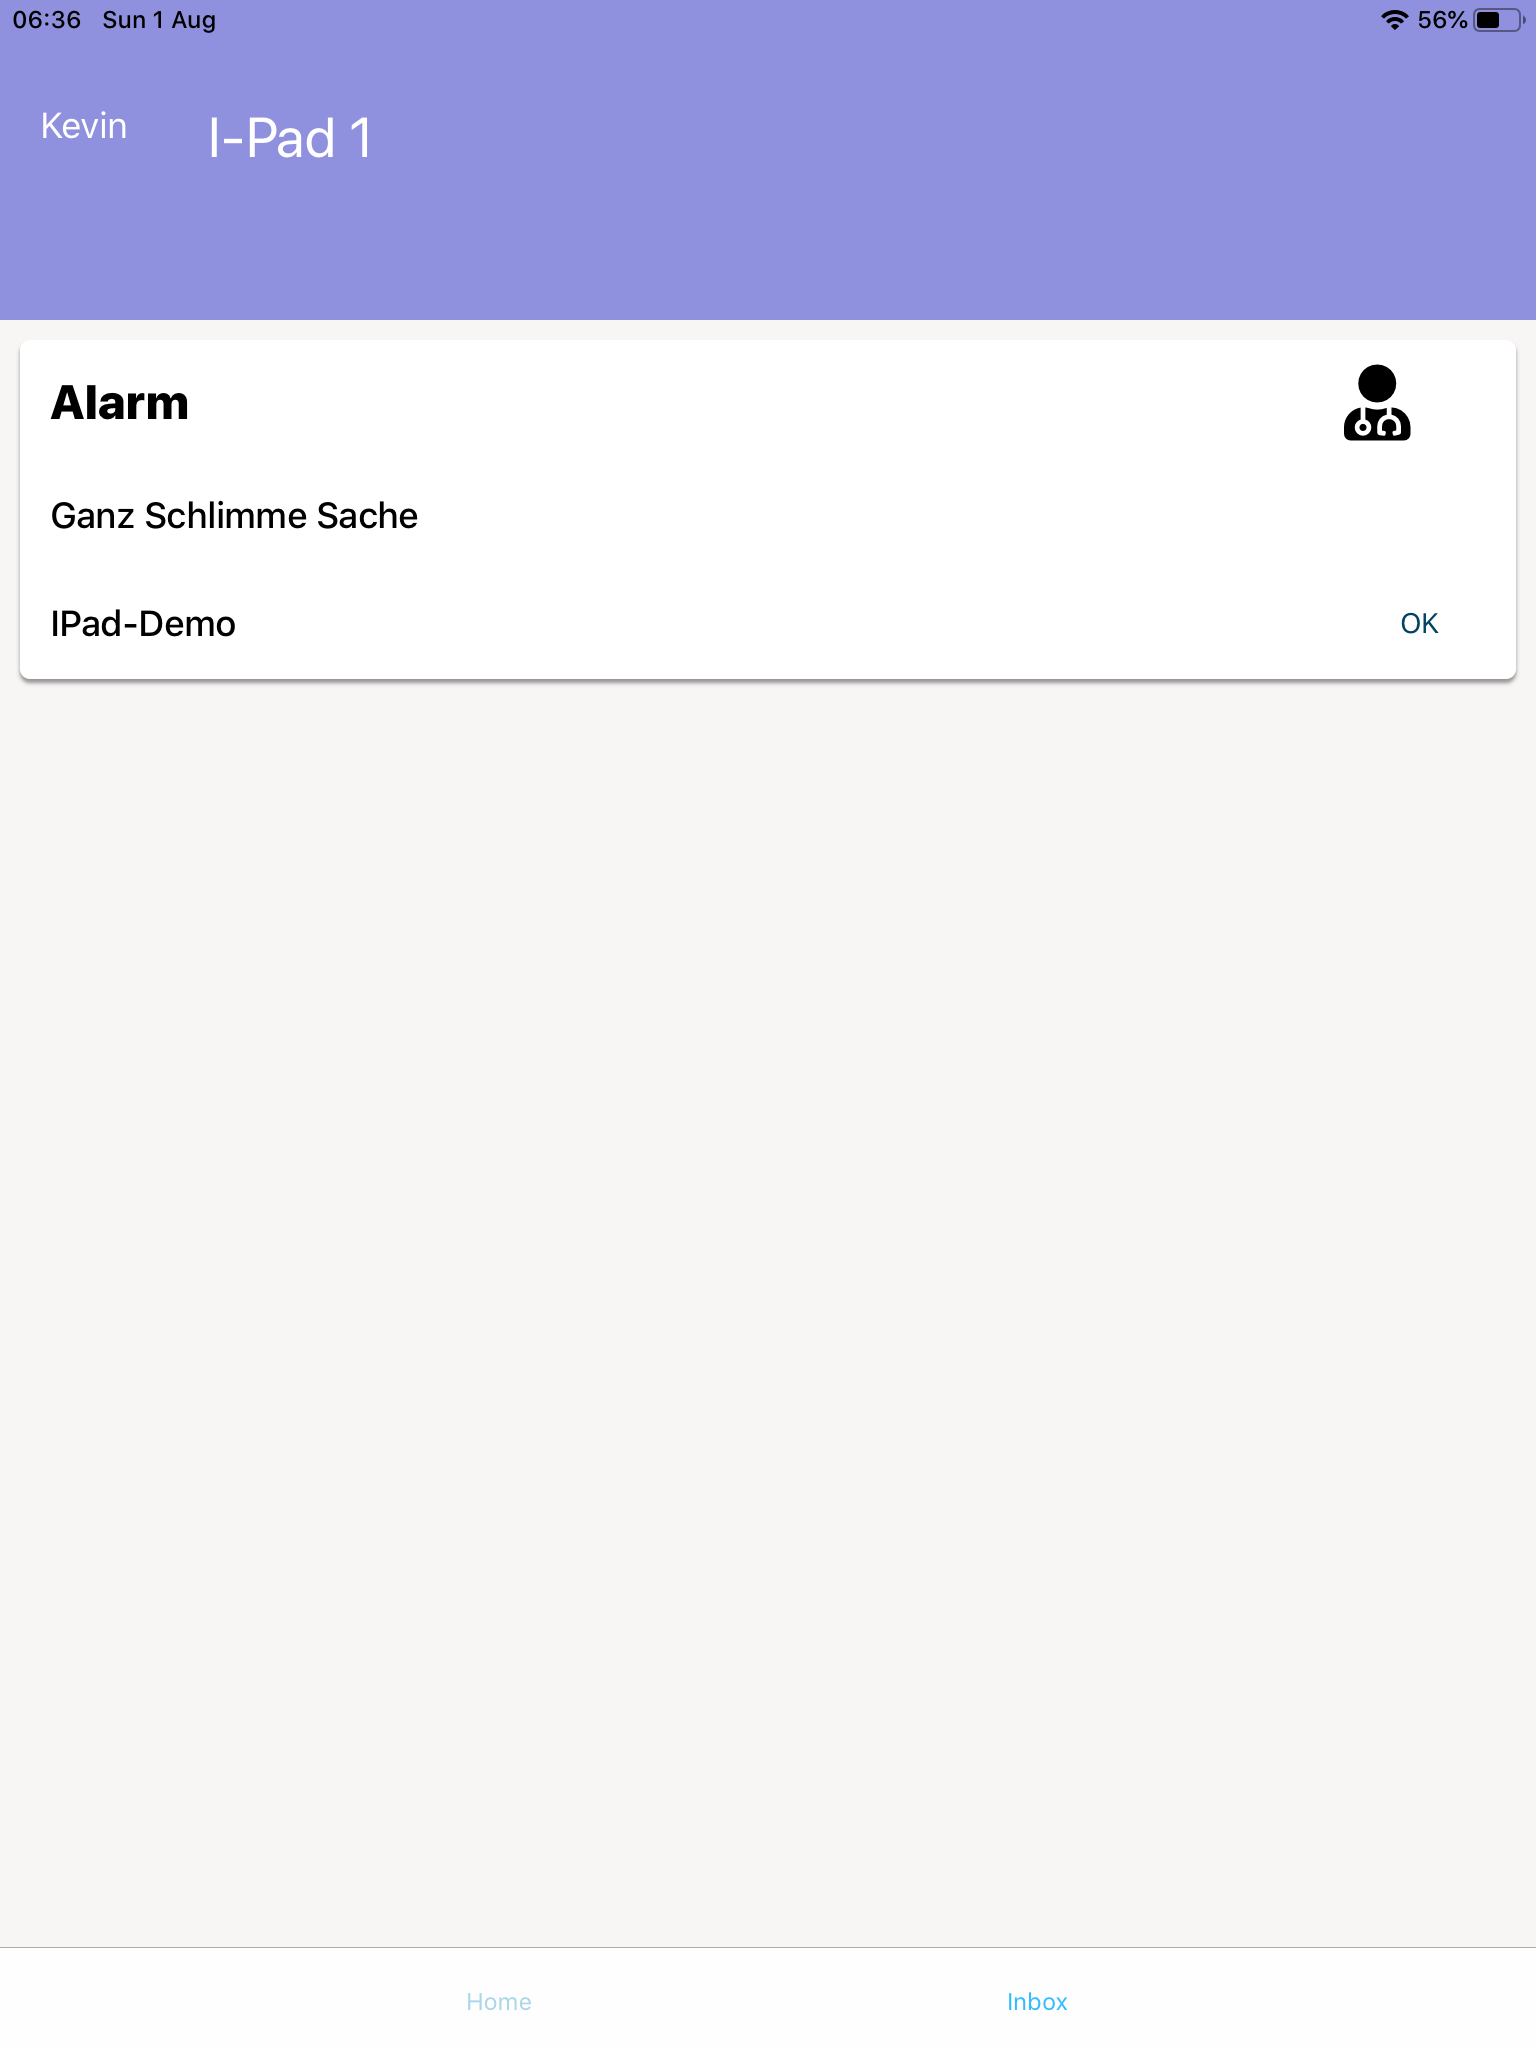
\includegraphics[width=\textwidth]{graphics/screenshots/mobileclient/screenshots-inbox}
        \caption{Retry}
    \end{minipage}
    \label{fig:MobileClient-Screens2}
\end{figure}

\clearpage

\subsubsection*{Benachrichtigungen empfangen}

Wurde eine Benachrichtigung empfangen, ertönt ein Audio Signal und die Benachrichtigung ist im Tab Inbox auf der Startseite ersichtlich.
Durch Klick auf einen der Einträge in der Liste, kann der Benutzer die empfangene Benachrichtigung quittieren.
Wenn die Inbox Benachrichtigungen enthält, die nicht quittiert wurden, wiederholt der Client im Abstand von 30
Die Quittierung von Benachrichtigungen erfolgt nur lokal auf dem Gerät.
Der Versender wird nicht über die Quittierung benachrichtigt.

Wurde eine Benachrichtigung im Hintergrund empfangen, wird diese als Push-Benachrichtigung auf dem Gerät angezeigt.
Auch wenn die Benachrichtigung im Hintergrund empfangen wurde, wird diese in der Inbox angezeigt.

\begin{figure}[h]
    \centering
    \begin{minipage}[b]{0.4\textwidth}
        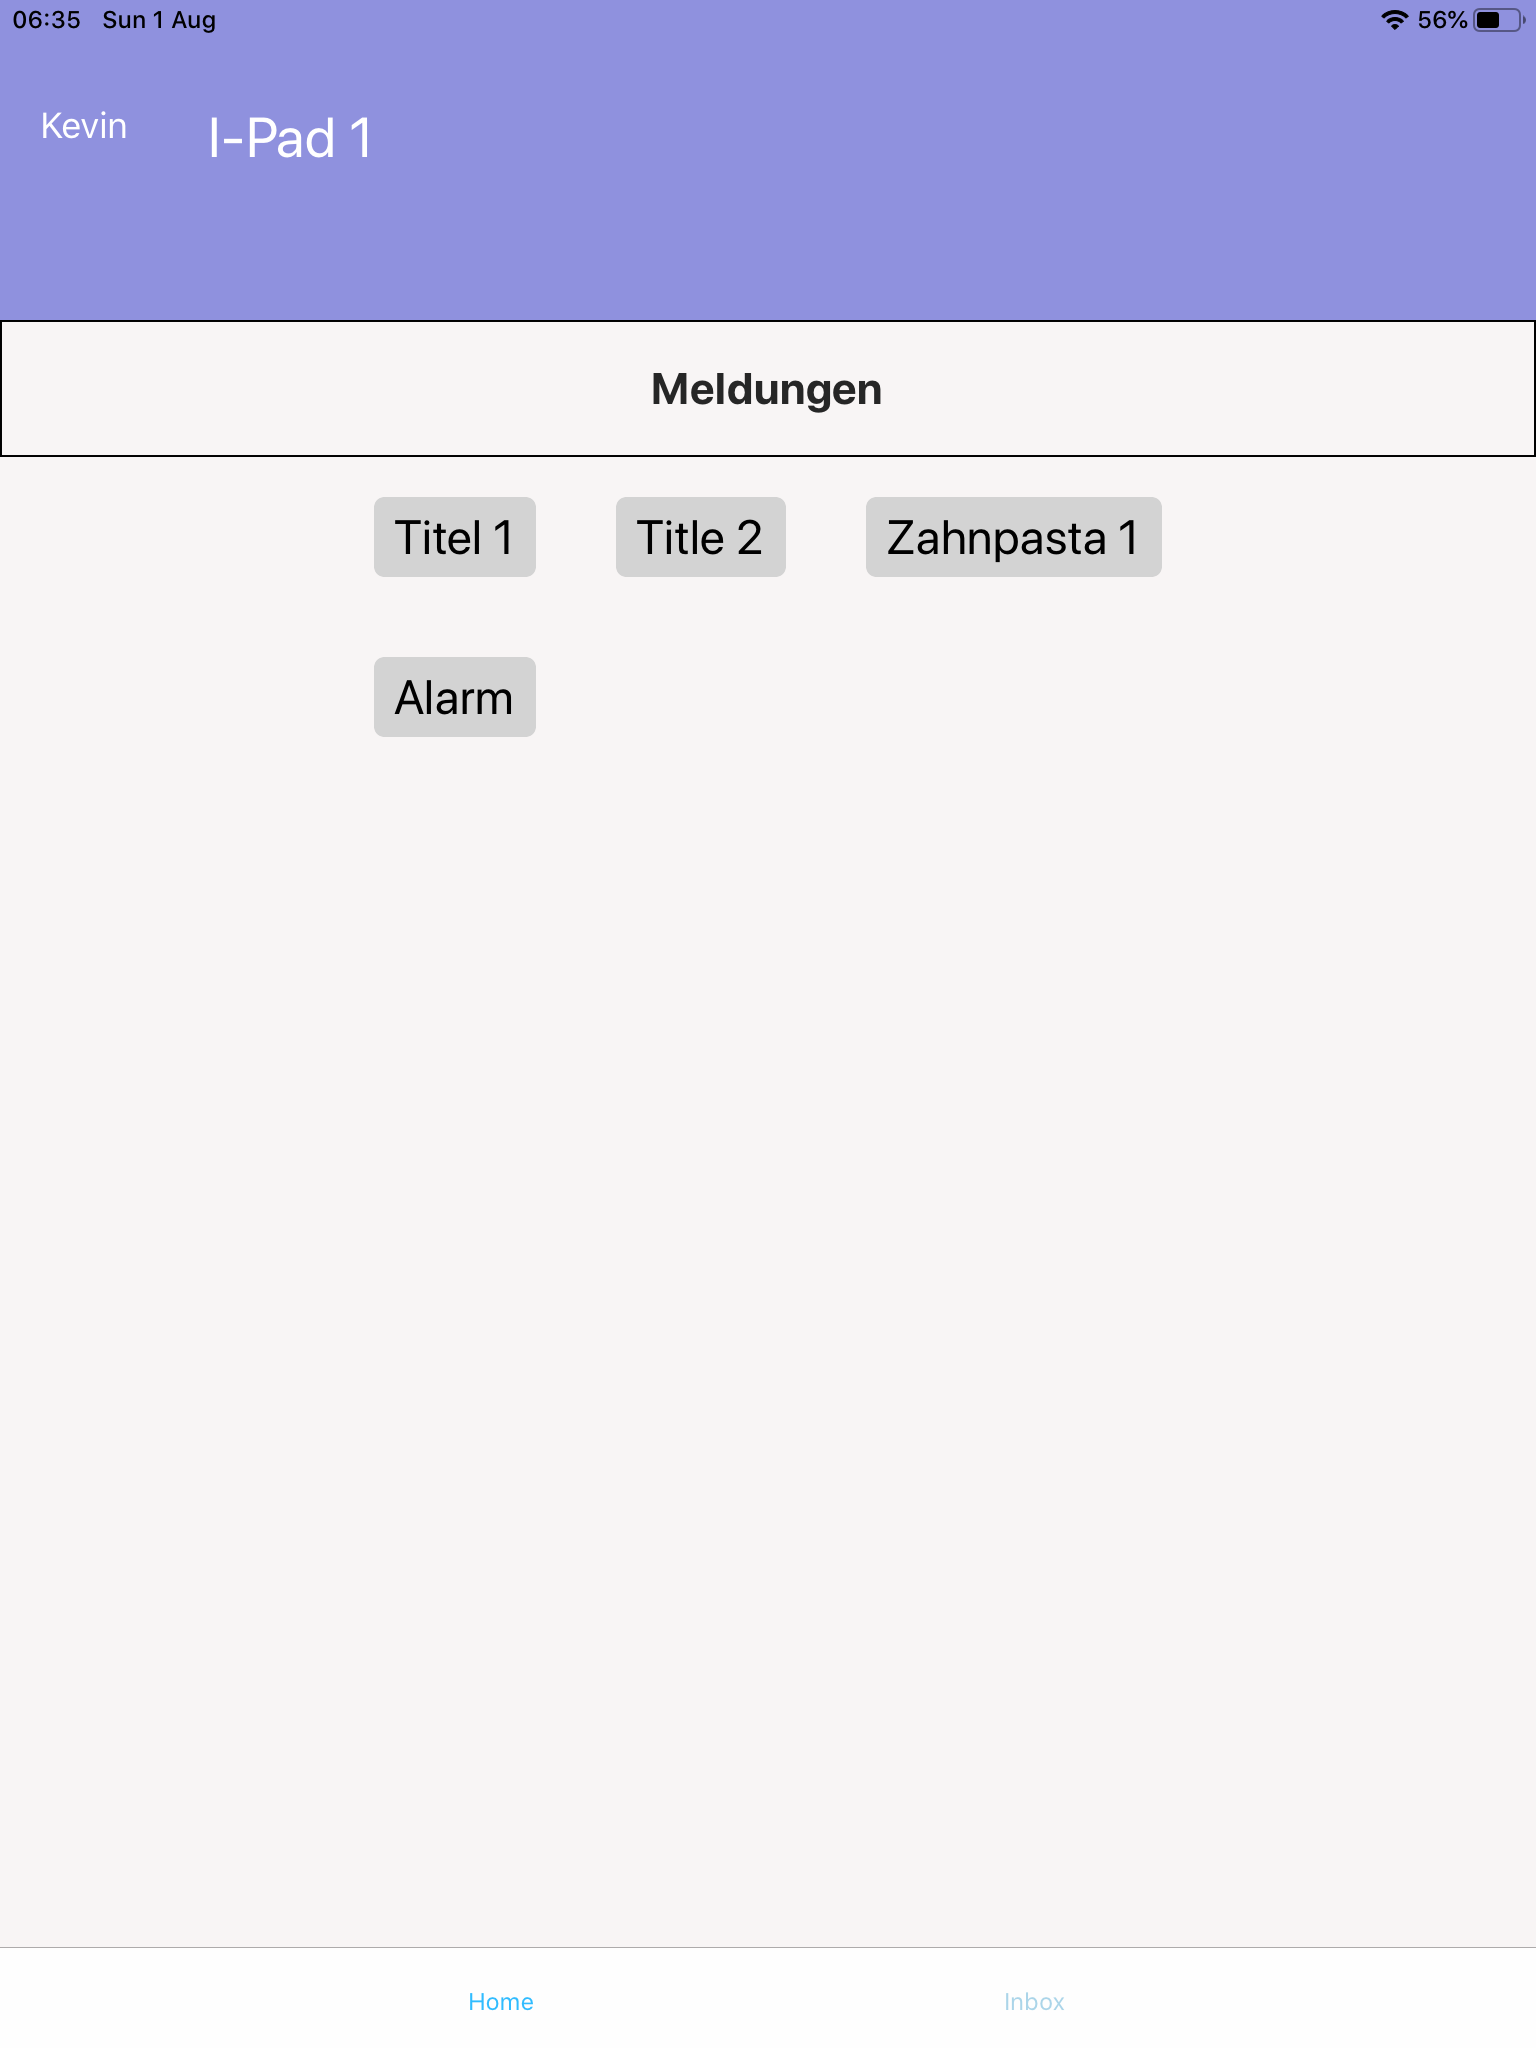
\includegraphics[width=\textwidth]{graphics/screenshots/mobileclient/screenshot-homescreen}
        \caption{Inbox}
    \end{minipage}
    \hfill
    \begin{minipage}[b]{0.4\textwidth}
        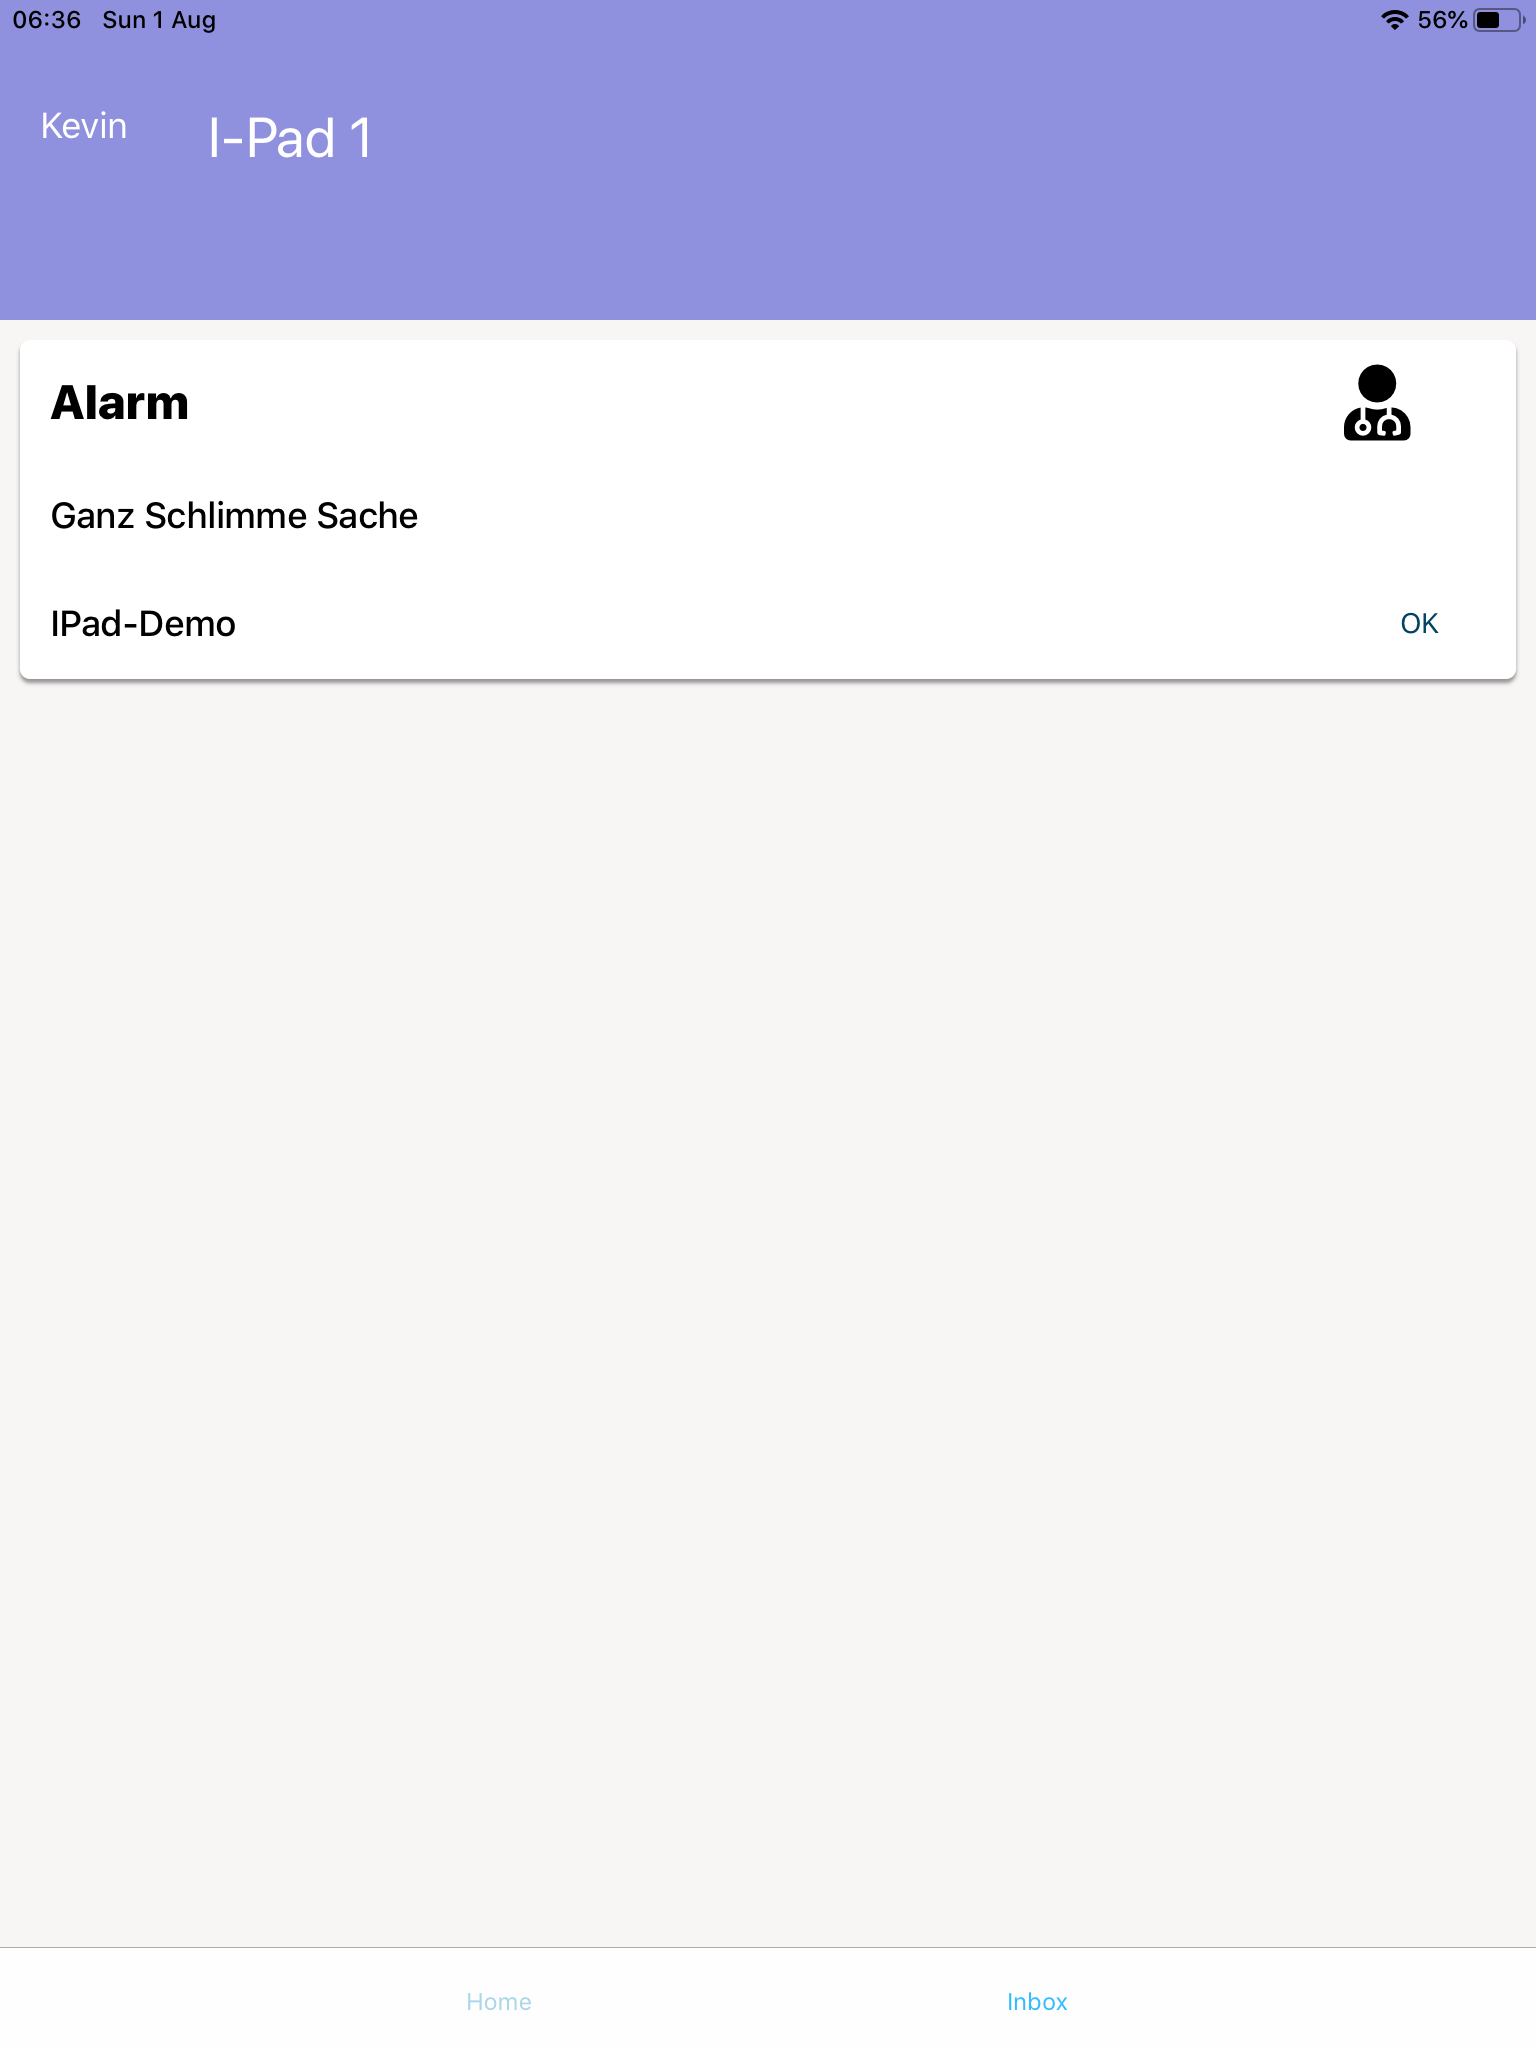
\includegraphics[width=\textwidth]{graphics/screenshots/mobileclient/screenshots-inbox}
        \caption{Push Benachrichtigung}
    \end{minipage}
    \label{fig:MobileClient-Screens3}
\end{figure}

%//TODO: Please replace second home screenshot with  Screenshot of push notification beeing displayed

\clearpage

